\documentclass[main.tex]{subfiles}
\begin{document}
  \section{Evaluating the Model}
      
      The model has been assessed by comparing it to data from real matches. \\
      In this process a small subset of data was dedicated as the "training" set, and used to adjust the model and inform modelling decisions. The remaining data was designated the "test" set that was used upon development completion to evaluate the model.
      
      \subsection{Data Aquision}
        
        Data was taken from Poland's Men's World Championship \cite{dataGames} by noting down relevant data in excel, based on the defined model. This was done early on in development, as mentioned previously. Specifically the data included the game's score, the coordinates the setter came in contact with the ball, the position the setter decided to set to, the success of the attack and mistakes that were made, among others.
        \\\\
        While this was done early in the development, it quickly became clear that a number of parameters, like mistakes in passing and sets from very difficult positions, were beyond the scope of the model. These phenomena involve a fair degree of rather unpredictable factors and would uunnecessarily complicate the model.
        \\\\
        Furthermore, from the impressions these games left it was possible to form design decisions, in particular those that fine tuned the model. For example, position 3 stands out by being extremely viable when the setter is close, but always being a bad choice when the setter is even slightly further away. This is different from other positions, that are generally still viable from slightly further away, and has to do with its central position, as the opponent can gang up on this position easily and quickly, unlike in other positions.\\
        
      \subsection{Analysis}
        
        The single most powerful description of the model's accuracy, quite obviously, is its ability to find the best position to set to. This should eb the position that is scored highest by the model, and ideally also the position the real world setter decides to set to.\\
        As there is real world data on what the setter would have considered the second best choice at the time, this is largely the only parameter available to asses the accuracy of the model.
        \\\\
        For each prediction the model records whether the real setter's choice was scored highest (1), second highest (2) etc. This was dubbed the choice-rank.  
        \\\\
        discuss training and test graphs. These suggest that, similar to the central limit theorem, larger datasets move the curve closer a curve similar to the above one, and hence that the model holds.
        \\\\
        More precisely, the model accurately scores positions by the likelihood of the setter to decide to set to them.
        \\\\
        \begin{figure}[h!]
          \begin{subfigure}{0.5\linewidth}
            \centering
            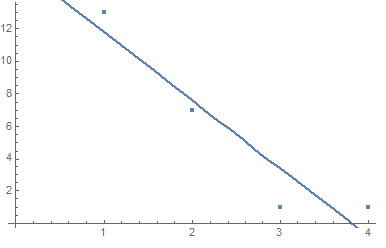
\includegraphics[width=0.9\linewidth]{figures/trainingGraph}
            \caption{text}
            \label{fig:training}
          \end{subfigure}
          \begin{subfigure}{0.5\linewidth}
            \centering
            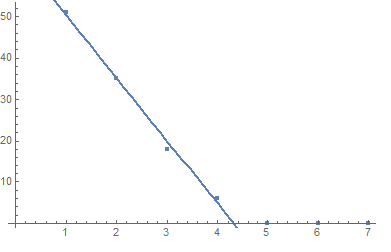
\includegraphics[width=0.9\linewidth]{figures/testGraph}
            \caption{text}
            \label{fig:test}
          \end{subfigure}
          \caption{text}
          \label{fig:analysis}
        \end{figure}
      
        
      All data used for the model was taken from the volleyball games in 2018 FIVB Men’s World Championships as they were available in high quality. Data acquisition consisted of watching the games where Poland played and recorded every decision the setter Fabian Drzyzga made from service reception. His position was recorded whenever he contacted the ball by pausing the game then estimating his coordinates.  For that reason, it was decided to split the court into a grid made out of squared meters as this reflects to which degree of accuracy the setter’s position during contact with the ball could be estimated to. The success rate of each set was also noted by determining if that set resulted with the point scored by the attacker. It is assumed that at this level all sets are good and there is no error in setting the ball. For the same reason the only sets that where counted where if the setter had enough time to get under the ball and use a volley to set rather then a dig. At international level if the setter can get behind the ball and use a volley all attacking option are possible however when using a dig there is a lot less control and precision therefore setter’s choices become drastically limited and very situational. For that reason, these sets where not counted. The points of both teams were also recorded during the set in order to correspond to the pressure factor. This point pressure encourages the setter to play more stable options and therefore the likelihood of more difficult plays in those moments decreases. The last thing that was noted was the position of the setter in the rotation. During service reception players “stack” in order to be in the most optimum receiving position while still following the rotation rules. This means the setter will start in different places meaning he might have to run further or closer to the pass.
    \subsection{Results}
      The model was tested by comparing how it behaves compared to the real data given exactly the same data. One hundred and ten different scenarios where fed into the model from the real data and then the setter’s decisions where compared to the actual ones. The choices are ranked 1st to 7th, 1st meaning that the real decision was predicted to be 1st in the model and 7th if the real decision was predicted to be 7th by the model. In order from 1st choice to the 7th choice out of 110 sets the model’s predictions are (51, 35, 18, 6, 0, 0, 0). In volleyball position 5 and the setter’s position (1 or 2 depending if the setter is backcourt or not) are not possible. Position 5 is a libero and the setter can not set himself. The 7th option is a tip were the setter attacks the ball instead of setting. This means that our model should never have any 7th or 6th ranked choices as it would mean its faulty. As it can be seen only 6 sets where ranked 4th by the model. To determine where this error was coming from, set distribution was represented in the following structure where for each individual position choices where listed from 1st to 7th.
Tip: (0, 0, 0, 0, 0, 0, 0)
Position 1 - Opposite Hitter back court: (3, 0, 6, 0, 0, 0, 0)
Position 2 – Opposite Hitter front court: (21, 8, 1, 0, 0, 0, 0)
Position 3 – Middle Hitter front court: (9, 11, 1, 0, 0, 0, 0)
Position 4 – Outside Hitter front court: (18, 15, 8, 0, 0, 0, 0)
Position 5 – Libero back court: (0, 0, 0, 0, 0, 0, 0)
Position 6 – Pipe Attack back court: (0, 1, 2, 6, 0, 0, 0)
From this data it is clear that Position 6 was incorrectly predicted by the model. The specific scenario from the real data that resulted in set to position 6 was checked and it turned out that position 6 was set 7/9 times from a perfect pass. Position 6 is back court which means it’s a lot harder to score a point from that position compared to from court positions. From the perspective of the model given a perfect pass it is really easy to set to front court positions which also have bigger success rate and are a lot easier and safer to set to then why would someone set backcourt in such scenario? Position 6 also known as pipe attack is very similar to timing with the middle attack (position 3). The set to pipe attack is very similar to the one in middle one apart from the fact is slightly higher and behind position 3. Because it is so similar to middle attack a lot of the time the blockers on the other side jump to block the middle player and end up falling down and landing just as the pipe attack happens meaning the pipe attack has no block therefore a higher chance of scoring. Given this nature of the pipe attack it most effective if the pass is perfect for a middle set. During such a perfect pass it only makes sense to set to middle as this position has the highest success rate out of all positions but is only possible on a good pass. Therefore, the block will end up most of the time jumping with the middle attack and that’s specifically why the setter would decide to go with the more unlikely set to the position 6 from time to time. This is incredibly difficult to predict as it does not happen often and since the model does not take opponents block and the whole ideal of fooling opponents block into the account it does not predict position 6 very well. The two times position 6 was set because of the pass being away from the net the model predicted it to be 2nd and 3rd choice which is no that bad as given those circumstances there is a very small difference in success rate between positions therefore each position has almost the same likelihood of being set to.  The next biggest inconsistency in the model is the position 4 with 15 2nd choices and 8 3rd choices. Position 4 is the safety position, meaning no matter how much pressure there is or how bad the pass is position 4 is pretty much always an option. It is also a position which is often preferable to set to from the perfect pass as 1 blocker often stays with the middle in those circumstances. Again, because the blocking is not considered by the model and the nature of that position being most of the time a viable option there is not much difference between 1st and 2nd options and it to certain degree it is often 50/50 which one will get set. Similar principle applies to position 3 which when is a viable option makes other positions also more viable because of the block distribution and therefore there will not be much difference between 1st and 2nd choices and that is reflected with the model predicting position 3 9 times correctly and 11 times as 2nd option. Only once the model predicted it as a 3rd option which is very good. Position 1 has 6 out of 9 sets as 3rd choice and since it is a back court position it is very likely that it was used to avoid the block for which the model does not account for. 

\end{document}